% Projekt: IFJ15 (Interpret jazyka) - prezentace
% Autor: Patrik Jurnečka
% Login: xjurne03
% Email: xjurne03@stud.fit.vutbr.cz
% Datum: 

\documentclass[pdf]{beamer}
% Preambule
\usetheme{Warsaw}
\usepackage[czech]{babel} %Jazyk
\usepackage[utf8]{inputenc} %Kodovani
\usepackage{graphics} %Obrazky
\usepackage{picture}

\title{Interpret imperativního jazyka IFJ15}
\subtitle{Tým 043, varianta b/2/I}
\author{Patrik Jurnečka}

\providecommand{\uv}[1]{\quotedblbase #1\textquotedblleft} %Uvozovky 


\begin{document} %Textova cast

\begin{frame}
	\titlepage
\end{frame}
	
\section{Interpret imperativního jazyka IFJ15}
\subsection{Složení týmu}
\frame {
	\frametitle{Složení týmu}
		\begin{itemize}
			\item Martin Honza
			\item Patrik Jurnečka
			\item Hana Slámová
			\item Frantisek Šumšal (vedoucí týmu)
			\item Adam Švidroň
		\end{itemize}
}

\frame {
	\frametitle{Obsah}
		\begin{enumerate}
			\item Organizace
			
			\item Lexikální analyzátor
			
			\item Syntaktická s sémentická analyzátor
			
			\item Interpret a páska instrukcí
			
			\item Funkce pro vyhledávání a řazení
			
			\item Práce v týmu
		
		\end{enumerate}
		
		\begin{figure}
			\scalebox{0.15}{\includegraphics{image.png}}
		\end{figure}
}

\frame{
	\frametitle{Organizace}
	\begin{enumerate}
		\item Zvolení vedoucího týmu
		\item Rozdělení práce na jednotlivé moduly
		\item Imlementace modulů 
		\item Testování
		\item Tvotba dokumentace
	\end{enumerate}
	
	\begin{figure}
		\scalebox{0.2}{\includegraphics{team.png}}
	\end{figure}
}

\frame {
	\frametitle{Lexikální analyzátor}
	\begin{enumerate}
		\item Vstup
			\begin{itemize}
				\item Zdrojový kód 
			\end{itemize}
			
		\item Výstup
			\begin{itemize}
				\item Posloupnost tokenů
			\end{itemize}
			
		\item Realizace
			\begin{itemize}
				\item Pomocí navrženého konečného automatu
			\end{itemize}
			
	\end{enumerate}
}

\frame {
	\frametitle{Konečný automat lexikální analyzy}
	
	\begin{figure}[h]
		\centering
		\scalebox{0.12}{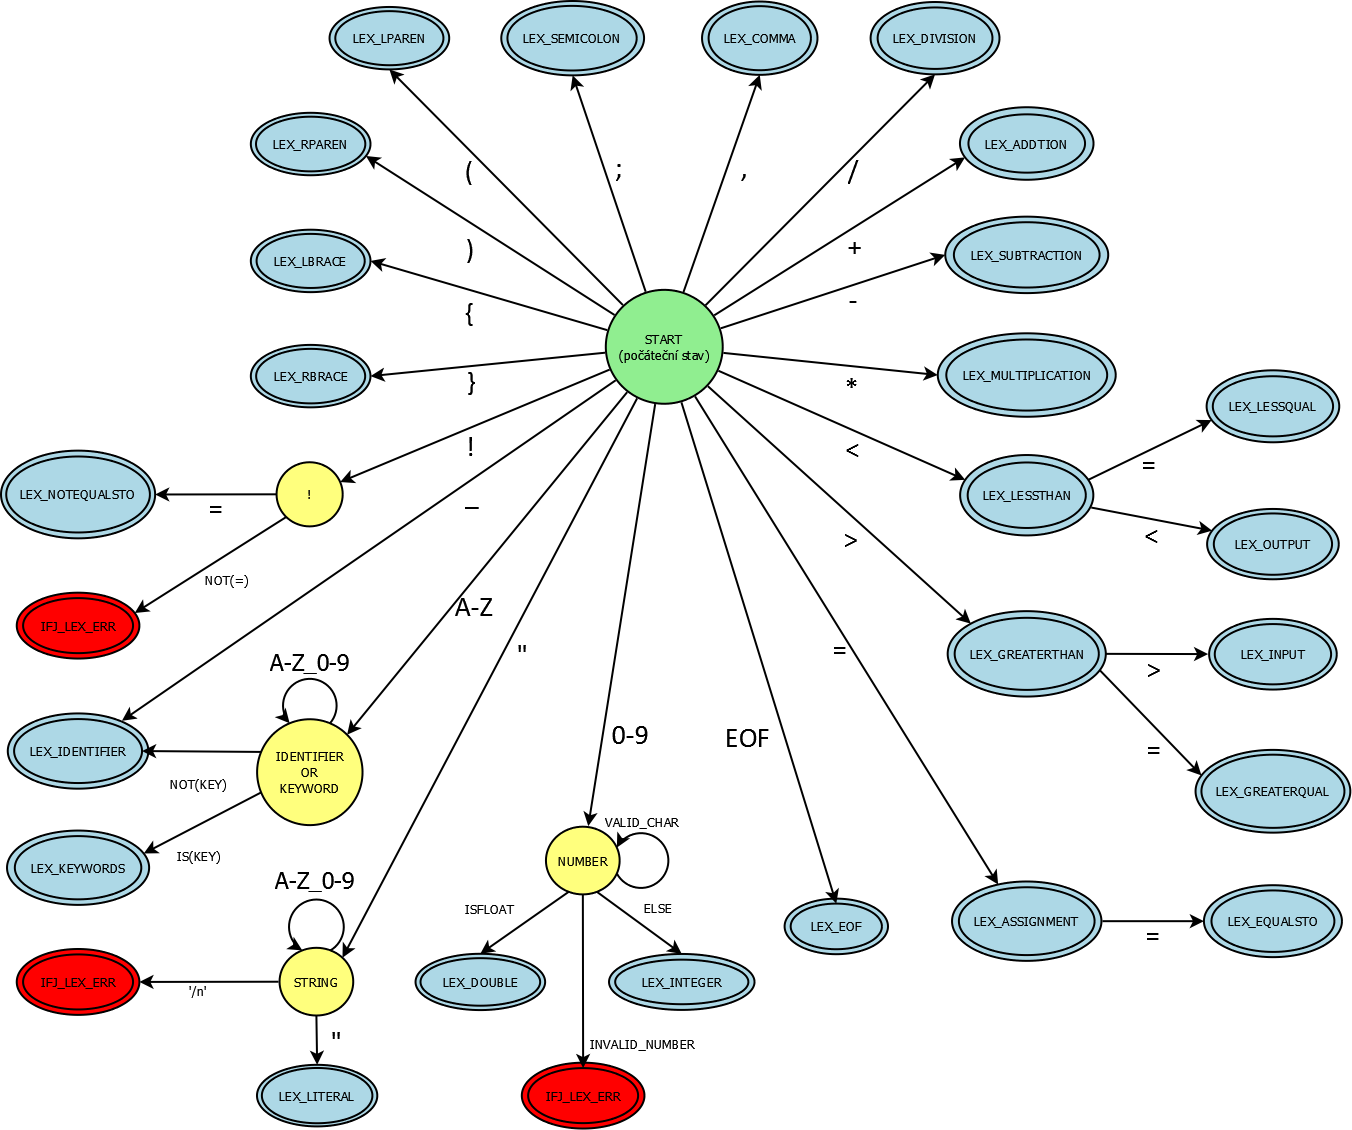
\includegraphics{konecny_automat.png}}
		\label{picture_1:konecny_automat}
	\end{figure}
}

\frame{
	\frametitle{Syntaktický a sémantický analyzátor}
	\begin{enumerate}
		\item Kontrola syntaxe (správná posloupnost tokenů)
		\item Volání funkce lex\_get\_token()
		\item LL gramatika
		\item Precedenční analýza
		\begin{itemize}
			\item Precedenční tabulka
			\item Generování 3AC (tříadresný kód)
			\item Sémantické kontroly
		\end{itemize}
	\end{enumerate}	
}

\frame {
	\frametitle{Interpret}
	\begin{enumerate}
		\item Zpracovaní instrukční sady
	\end{enumerate}
}

\frame {
	\frametitle{Konec}
	\begin{center}
		\bigskip \LARGE Prosím o dotazy \\
		\bigskip \Huge \texttt{Děkujeme za pozornost}
	\end{center}
	
}

\frame {
	\frametitle{REFERENCE}
	\small 	
	{
	\textsc {AHO, Alfred V.}, J. \textit{Compilers: principles, techniques,}. 2nd ed. Boston: Pearson/Addison Wesley, c2007, XXIV, 1009~s. ISBN 03-214-8681-1.\\
	\bigskip
	}	
}

\end{document} %konec textove casti